\begin{figure}[!t]
    \centering
    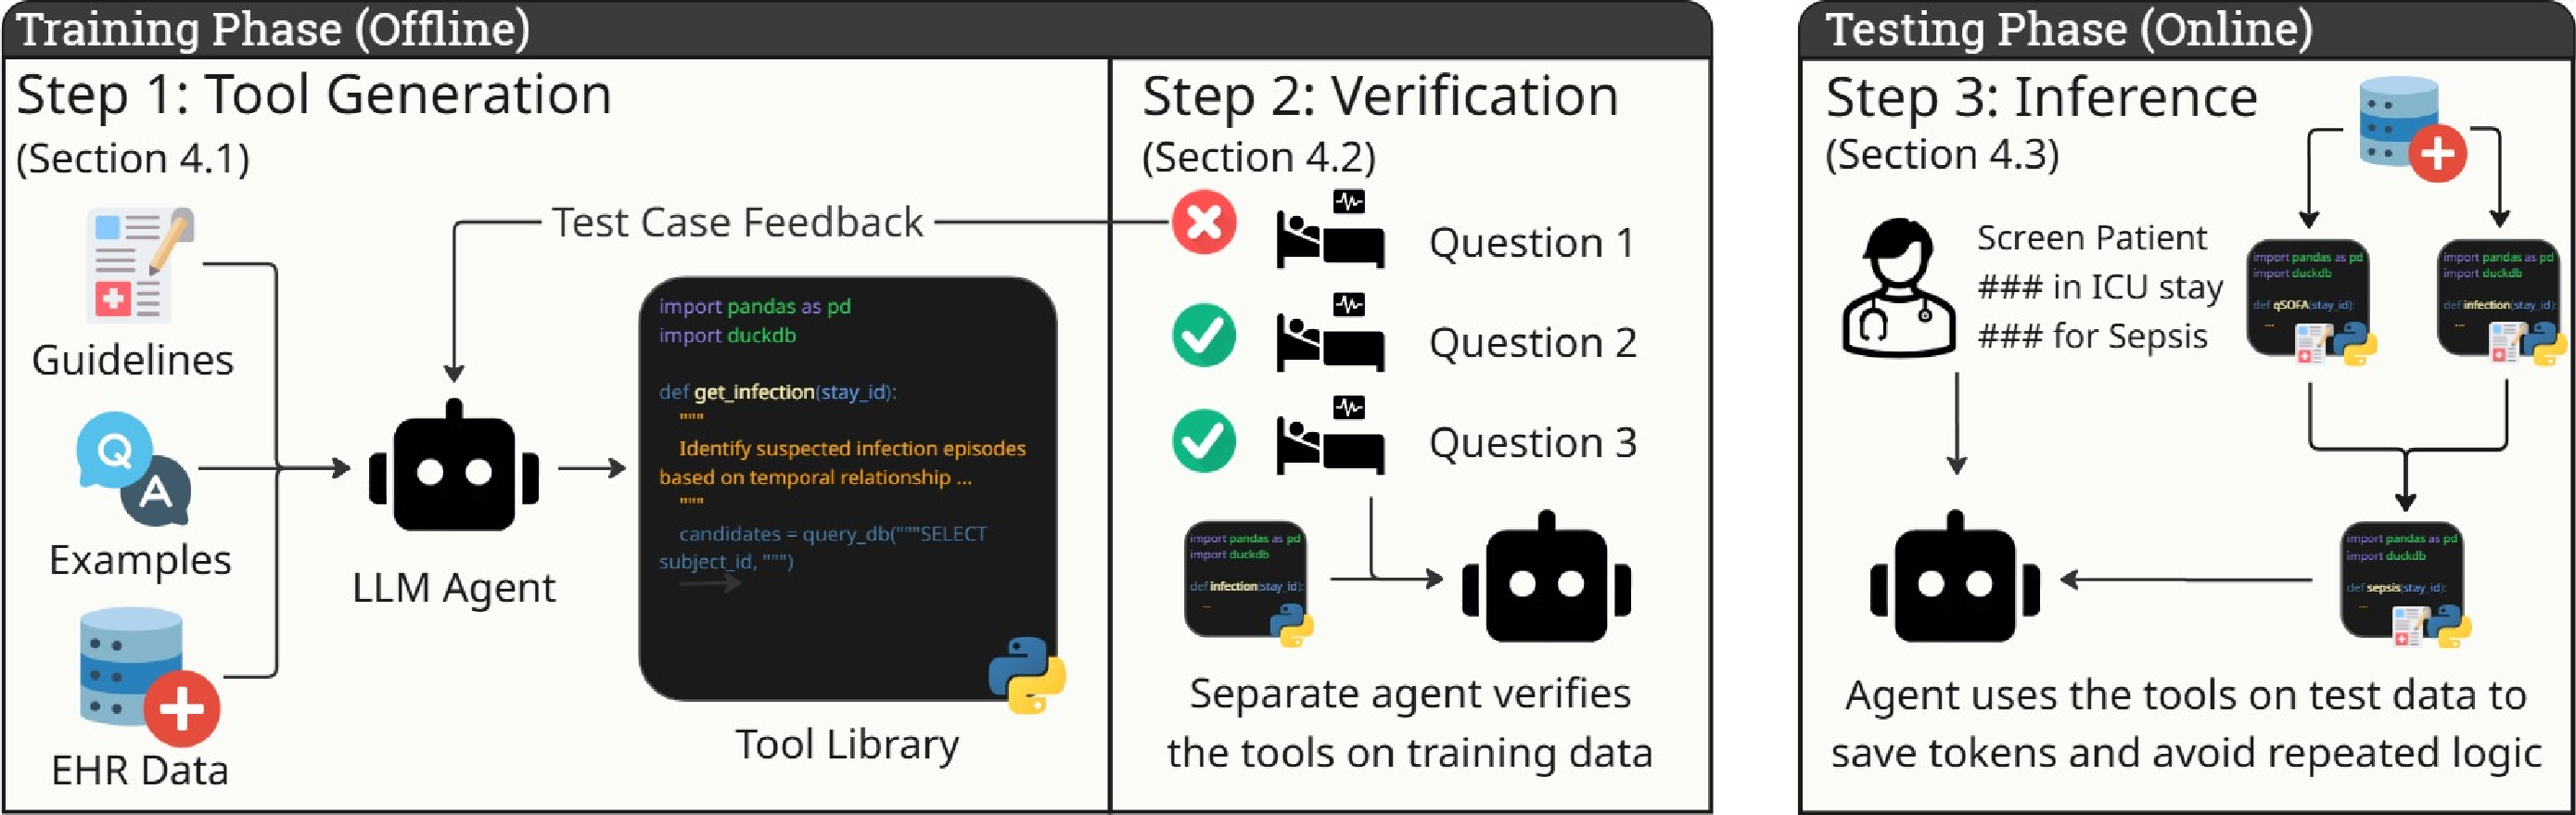
\includegraphics[width=\linewidth]{figures/pipeline.pdf}
    \caption{Overview of the clinical autoformalization pipeline. An LLM agent iteratively explores the EHR schema, consults clinical guidelines, and refines a Python function until it passes QA-based verification. Verified functions are stored in a shared library and reused compositionally for higher-level and new tasks.}
    \label{fig:pipeline}
\end{figure}

\begin{figure}[!h]
    \centering
    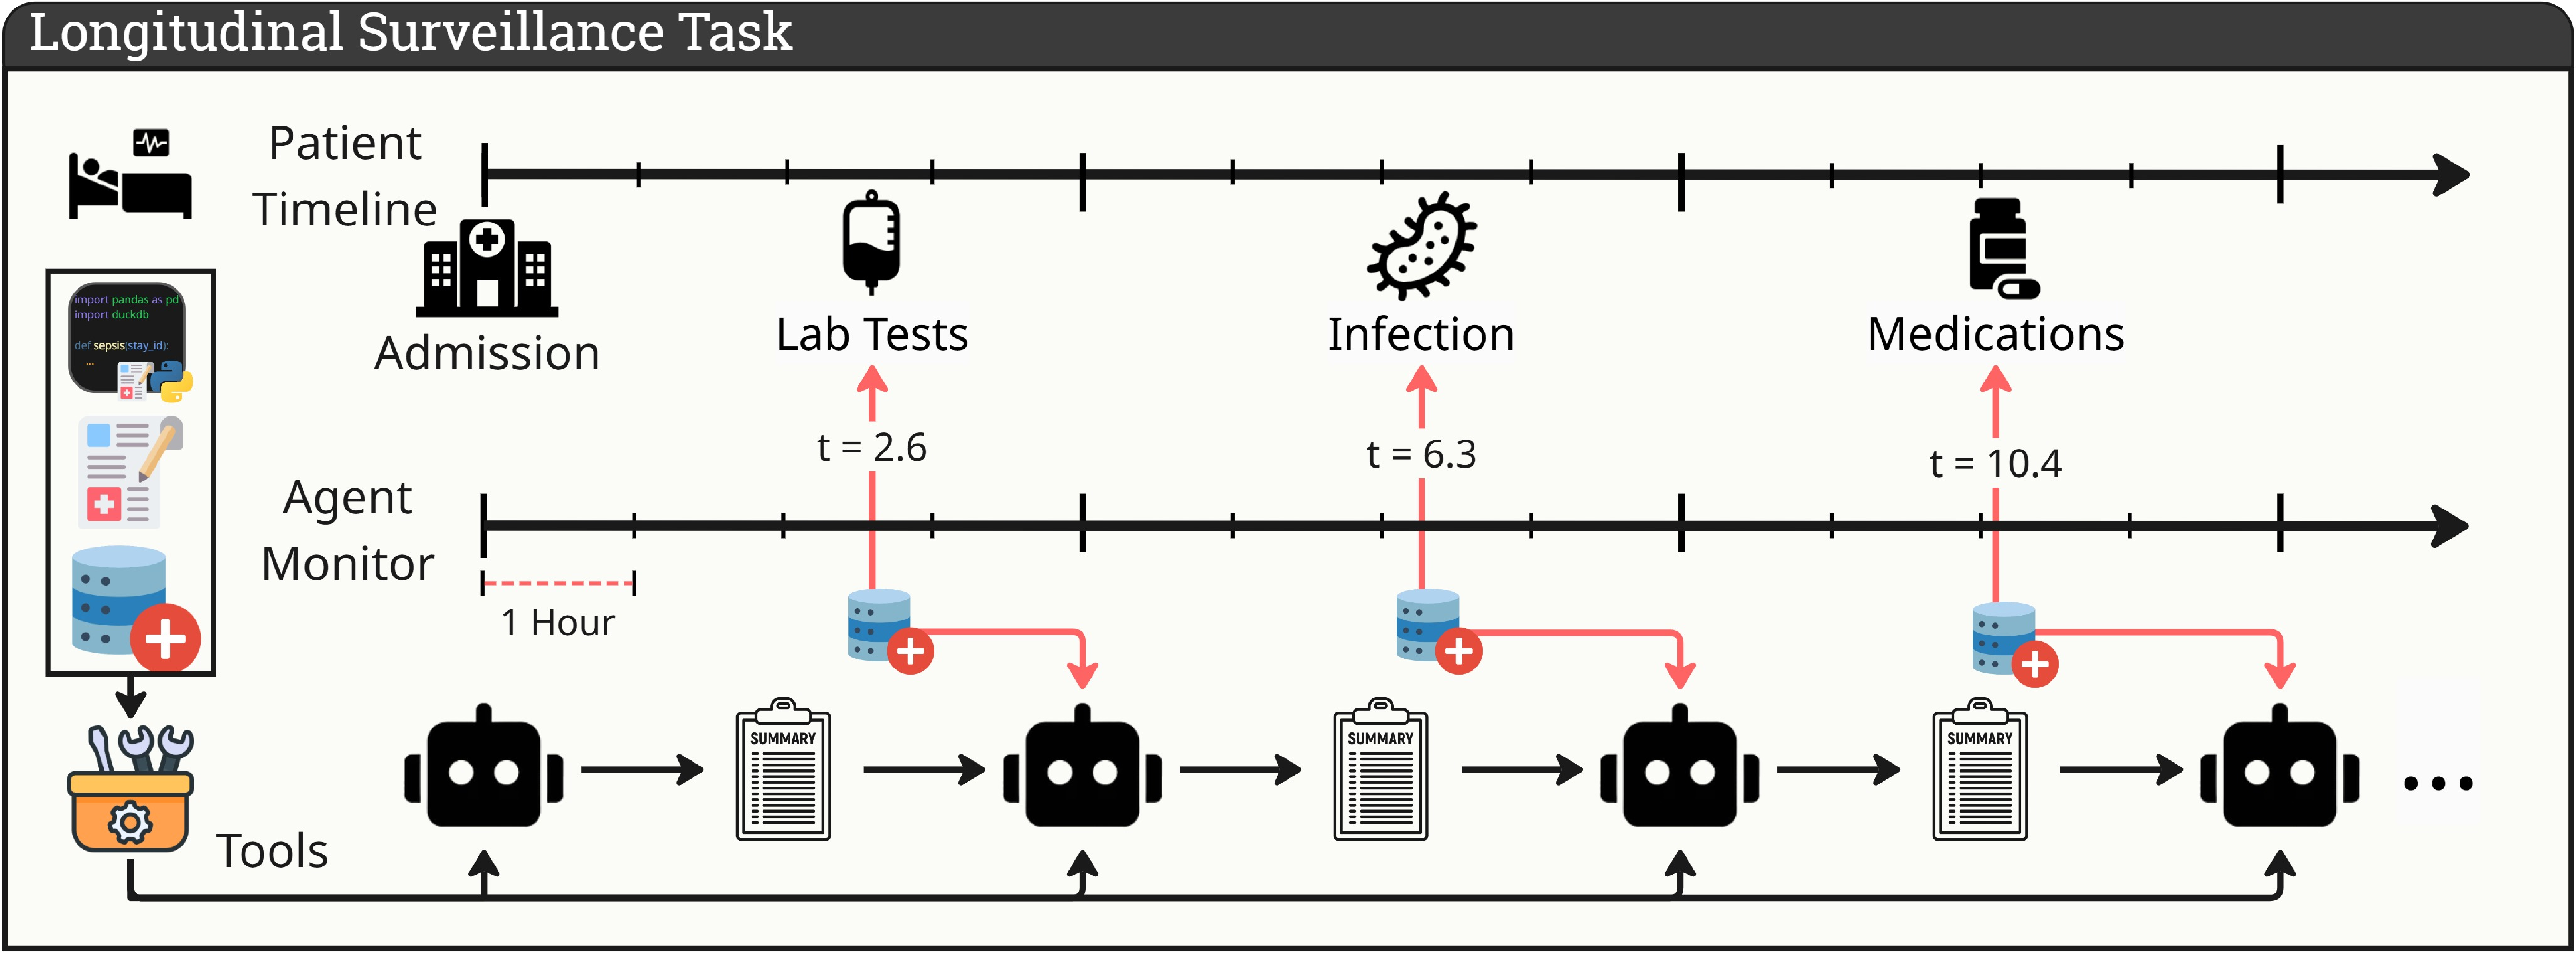
\includegraphics[width=\linewidth]{figures/longitudinal_pipeline.pdf}
    \caption{Overview of the longitudinal patient surveillance task in our benchmark. The LLM agent is prompted every 4 hours to predict patient condition and summarize.}
    \label{fig:longitudinal}
\end{figure}


\section{Baseline: Clinical Autoformalization}


We propose a clinical autoformalization pipeline that converts natural-language clinical guidelines into a verified, reusable Python function library using only a small train split as supervision. The pipeline takes as input a QA dataset $\mathcal{Q} = \{(q_k, y_k)\}_{k=1}^{K}$, an EHR database $\mathcal{C}$, and clinical guidelines $\mathcal{G}$, and produces a verified Python function $f$ that deterministically extracts a clinical concept for any patient. The full algorithm is given in Appendix~\ref{app:algorithm}.

\subsection{Tool Generation}

The core of the pipeline is an iterative ReACT loop~\cite{yao2023react} in which an LLM agent explores the EHR database schema, consults clinical guidelines, and writes a Python function for a target concept. The agent operates within a stateful code interpreter exposing three tools: \texttt{query\_db(sql)} for database access, \texttt{search\_guidelines}/\texttt{get\_guideline} for retrieving clinical specifications from $\mathcal{G}$, and \texttt{search\_functions}/\texttt{load\_function} for discovering and importing previously verified functions. Guidelines are exposed as a searchable library rather than injected into the prompt, forcing the agent to bridge clinical knowledge and database schema through autonomous exploration.

Concepts are processed in topological order over the dependency graph $G = (V, E)$, where $(v_i, v_j) \in E$ means $v_j$ depends on $v_i$. Leaf concepts are autoformalized first; higher-level concepts can then call previously verified functions as building blocks rather than reimplementing their logic. For example, when generating a function for \texttt{sepsis3}, the agent can load verified functions for \texttt{sofa} and \texttt{suspicion\_of\_infection} directly.

\subsection{Verification}

Once the agent produces a candidate function $f_t$, it is evaluated against the 10\% train split of $\mathcal{Q}$. A separate QA agent calls $f_t$ in its own code interpreter and parses a verdict for each question to compare against ground truth. If accuracy exceeds $\theta = 0.90$, the function is accepted and saved to the shared library. Otherwise, per-question error traces are fed back to the autoformalization agent as structured feedback for the next iteration. The best-performing candidate across all iterations is retained, so the pipeline is robust to minor regressions between steps.

\subsection{Inference}

Once the library $\mathcal{L} = \{f_1, \dots, f_M\}$ is complete, it is deployed as a static resource over the held-out 90\% test split. An LLM inference agent receives a clinical question $q$ along with access to $\mathcal{L}$ and the database, calls the relevant pre-verified functions according to its judgment, and reasons over their outputs to produce an answer:
\begin{equation}
    \hat{y} = \text{LLM}\bigl(q,\; \{f_j(p) : f_j \in \mathcal{L}\},\; \mathcal{C}\bigr)
\end{equation}
Because the functions in $\mathcal{L}$ have been verified on labeled cases, the inference agent's context is occupied by compact function signatures rather than raw schema exploration, substantially reducing token usage. The same function produces identical output for the same patient across runs, which is critical for reproducibility in clinical settings.
